%%%%%%%% ICML 2025 TEMPLATE USED FOR THIS PAPER %%%%%%%%%%%%%%%%%

\documentclass{article}

\usepackage{microtype}
\usepackage{graphicx}
\usepackage{subfigure}
\usepackage{booktabs} % for professional tables

% hyperref makes hyperlinks in the resulting PDF.
\usepackage{hyperref}


% Attempt to make hyperref and algorithmic work together better:
\newcommand{\theHalgorithm}{\arabic{algorithm}}

% Use the following line to anonymize the paper for peer review:
\usepackage{icml2025}

% For non-anonymized release, use this instead:
%\usepackage[accepted]{icml2025}

% For theorems and such
\usepackage{amsmath}
\usepackage{amssymb}
\usepackage{mathtools}
\usepackage{amsthm}

% if you use cleveref..
\usepackage[capitalize,noabbrev]{cleveref}

%%%%%%%%%%%%%%%%%%%%%%%%%%%%%%%%
% THEOREMS
%%%%%%%%%%%%%%%%%%%%%%%%%%%%%%%%
\theoremstyle{plain}
\newtheorem{theorem}{Theorem}[section]
\newtheorem{proposition}[theorem]{Proposition}
\newtheorem{lemma}[theorem]{Lemma}
\newtheorem{corollary}[theorem]{Corollary}
\theoremstyle{definition}
\newtheorem{definition}[theorem]{Definition}
\newtheorem{assumption}[theorem]{Assumption}
\theoremstyle{remark}
\newtheorem{remark}[theorem]{Remark}

% Todonotes is useful during development; simply uncomment the next line
%    and comment out the line below the next line to turn off comments
%\usepackage[disable,textsize=tiny]{todonotes}
\usepackage[textsize=tiny]{todonotes}


% The \icmltitle you define below is probably too long as a header.
% Therefore, a short form for the running title is supplied here:
\icmltitlerunning{Evaluating the Impact of Randomized Sampling on Diverse Prediction Model Training}

\begin{document}

\twocolumn[
\icmltitle{Evaluating the Impact of Randomized Sampling on Diverse Prediction Model Training}

% You can specify symbols, otherwise they are numbered in order.
% Ideally, you should not use this facility. Affiliations will be numbered
% in order of appearance and this is the preferred way.
\icmlsetsymbol{equal}{*}

\begin{icmlauthorlist}
\icmlauthor{Luiz Parente}{equal,lp}
\end{icmlauthorlist}

\icmlaffiliation{lp}{School of Electrical and Computer Engineering, Purdue University, IN, USA}
\icmlcorrespondingauthor{Luiz Parente}{lparente@purdue.edu}

% You may provide any keywords that you
% find helpful for describing your paper; these are used to populate
% the "keywords" metadata in the PDF but will not be shown in the document
\icmlkeywords{Machine Learning, Sampling Algorithm, Leverage Scores}

\vskip 0.3in
]

% this must go after the closing bracket ] following \twocolumn[ ...

% This command actually creates the footnote in the first column
% listing the affiliations and the copyright notice.
% The command takes one argument, which is text to display at the start of the footnote.
% The \icmlEqualContribution command is standard text for equal contribution.
% Remove it (just {}) if you do not need this facility.

%\printAffiliationsAndNotice{}  % leave blank if no need to mention equal contribution
\printAffiliationsAndNotice{\icmlEqualContribution} % otherwise use the standard text.

\begin{abstract}

In the modern world, data generation and collection have become ubiquitous, and machine learning algorithms are constantly employed to implement intelligent models for a diverse range of practical use-cases. Large corporations leverage customer data to predict consumption patterns. Health practitioners utilize medical datasets to diagnose sickness. Social media companies parse through \textit{likes} and \textit{comments} to analyze human behavior and maximize user engagement.

The reliance on big-data has increasingly become the norm. However, as the available data grows in size and dimensionality, the computational power required to train such models increase proportionally. Therefore, optimizing compute efficiency when leveraging large-scale datasets to train machine learning prediction models becomes an obvious necessity as society shifts toward data-driven business models and paradigms.

This study focuses on exploring \textbf{data sampling} as a possible solution for the problem of training on large data. The goal, given a dataset, is to derive a smaller subset that retains the main characteristics of the whole, allowing for the training of prediction models that provide comparable accuracy to those trained on the full dataset, however at a lower training cost.

\end{abstract}

\section{Literature Review}
\label{submission}

\subsection{Background}

\textbf{Logistic regression} is a supervised learning technique commonly used to model the probability of an event occurring based on predictor variables. In the field of Machine Learning, logistic regression is often applied in the context of disease classification, anomaly detection, among others.

Despite being a well established and effective method for binary classification use-cases, handling large-scale datasets often present unique computational and algorithmic challenges, particularly in terms of time and space complexity, that demand specialized solutions. For example, logistic regression models typically employ optimization methods such as gradient descent to find the best-fitting parameters. The computational cost of each iteration is proportional to the number of observations and the number of features, often times making the optimization procedure computationally expensive.

With large datasets, the time complexity can become prohibitive, as the number of operations required for each iteration increases. Additionally, many logistic regression implementations require storing the data-points and intermediate computation results in memory. When working with big-data, this approach can lead to hardware bottlenecks. In particular, storing and manipulating large feature matrices can demand significant amounts of random-access memory (RAM), especially when the number of features is substantial. When the dataset exceeds memory limits, performance can degrade significantly, requiring the use of additional tooling, such as distributed computing or data sampling, as a means to overcome such challenges.

\subsection{Problem Definition}

This work aims to explore potential solutions to the computational challenges posed by the use of high-dimensional datasets in the context of prediction models. Objectively, we evaluate the impacts, implementations, and viable utilizations for a randomized sampling algorithm originally designed for logistic regression models, as outlined by \citet{chow24}. Given a dataset, the proposed method derives a smaller subset that retains the most representative data-points, using it to train a prediction model capable of achieving accuracy levels comparable to models trained on the entire dataset. As demonstrated both theoretically and experimentally, the algorithm is successful at substantially reducing the size of training datasets, addressing many barriers found when handling large databases in machine learning applications.

Given the predominance of digital systems driven by big-data in modern society, investigating implementation variations and applicability potential is a justified effort, and may help to further understand possible trafe-offs between algorithmic simplicity and prediction accuracy, as well as effectiveness in diverse data configurations.


\subsection{Summary and Critique of the Selected Papers}

\subsubsection{Main Paper: A Provably Accurate Randomized Sampling Algorithm for Logistic Regression \cite{chow24}}

\textbf{Summary:} Logistic regression is a widely used method for binary classification tasks, where the goal is to predict one of two possible outcomes based on input features \cite{pml}. However, when the number of observations greatly exceeds the number of predictor variables, solving logistic regression becomes computationally expensive. In this work, \citeauthor{chow24} propose a novel approach to address this issue by leveraging a randomized sampling technique that guarantees high-quality approximations to the estimated probabilities of logistic regression, with a sample size significantly smaller than the total number of observations. The primary goal is to make logistic regression more computationally efficient for large-scale datasets while maintaining prediction accuracy.

The paper focuses on the use of leverage scores, which is a method that, given a dataset, allows for the extraction of a subset where the derived data points retain the main characteristics of the overall data \cite{ordo22}. The authors' proposed algorithm constructs a sampling matrix using these scores, and the resulting subsampled log-likelihood function is optimized to estimate the model parameters. This randomized approach allows for substantial reductions in computational cost while preserving the accuracy of the regression model.
The paper provides a theoretical derivation of an approximation bound that guarantees the accuracy of the estimated probabilities obtained from the subsampled data. This result is significant because it shows that only a small subset of the data may be needed to achieve a high-quality approximation of the original data, making the algorithm more scalable and efficient.

To validate their approach, the authors conduct extensive empirical evaluations on real-world datasets, including a cardiovascular disease prediction dataset, a customer churn prediction dataset, and a credit card default prediction dataset. The experiments compare the performance of the proposed leverage score-based sampling method with other sampling schemes, including uniform sampling and the L2S method proposed by \citeauthor{mun18}. The results demonstrate that the leverage score-based method performs comparably to other methods in terms of the accuracy of estimated probabilities, and shows potential for outperformance, particularly as the sample size increases. Moreover, the method achieves misclassification rates close to those obtained by the full-data model, further confirming its effectiveness. These empirical results validate the theoretical claims and show that the proposed algorithm can deliver accurate logistic regression estimates with a reduced sample size.

The paper concludes with a discussion about the implications of their findings and suggesting future research directions. While the proposed method performs well in practice, the authors highlight that there is still room for improvement in terms of algorithmic efficiency and scalability, particularly in high-dimensional settings. They also suggest exploring alternative sketching techniques, such as random projection-based methods, to further enhance the sampling process. Additionally, the paper points out that the approach could be extended to handle other forms of regression and machine learning models, making it a valuable tool for a variety of applications. The paper makes a significant contribution by providing an efficient and scalable solution to logistic regression for large datasets, with strong theoretical guarantees and solid empirical results.

\textbf{Critique:} While the paper provides an excellent approach for logistic regression, it does not explore the application of the same sampling algorithm to other types of prediction models. The authors focus exclusively on logistic regression, which is understandable given the complexity and computational challenges associated with large datasets in this context. However, the question of whether the method could potentially be adapted for use with other models, such as linear regression, support vector machines, or even more complex deep learning models, remain unclear. Given that dataset distillation has been an area of interest in machine learning \cite{liu23}, a discussion of how their technique could be generalized or modified for broader applications range would have added valuable insight to the work. Exploring the adaptability of the sampling strategy to a range of prediction models could increase the impact and versatility of the proposed method, making it applicable to a wider array of real-world problems.

Additionally, even though the paper does provide a robust theoretical foundation for the proposed method, it could benefit from a more detailed exploration of the trade-offs between simplicity and accuracy, particularly when it comes to the complexity of the algorithm. While the proposed algorithm is presented as computationally efficient, the authors do not thoroughly investigate alternative variations of the algorithm that might provide different levels of complexity or accuracy. For example, they focus heavily on the use of row leverage scores to select data points, but it would be valuable to see whether simpler strategies could yield comparable performance. Moreover, a discussion of whether implementing theoretical guarantees—such as the approximation bounds—justifies the added complexity would provide a clearer understanding of the practical trade-offs involved. The paper does an excellent job of presenting an efficient solution, but more emphasis on evaluating the balance between theoretical rigor and real-world applicability could enrich the findings.

Another area where the paper could expand is in providing a more nuanced analysis of the error bounds and their impact on the overall model performance. While the theoretical guarantees are a key strength of the paper, there is limited exploration of how these bounds manifest in practice when applied to different types of datasets. It would have been helpful for the authors to conduct experiments that show how varying the sample size and error tolerance affects both the accuracy of the model and the computational efficiency. In addition, the relationship between the size of the dataset, the model's complexity, and the effectiveness of the approximation would have benefited from further elaboration. For example, is there a point at which the error bounds no longer provide substantial improvements, or do they continue to yield significant benefits with increasing complexity? Addressing these questions could further clarify when and why this sampling-based approach is most beneficial, providing a more comprehensive evaluation of its utility in real-world applications.


\subsubsection{Supplementary Paper: SLOE: A Faster Method for Statistical Inference in High-Dimensional
Logistic Regression \cite{yad21}}

\textbf{Summary:} In high-dimensional problems, where the number of features is comparable to or exceeds the number of samples, traditional logistic regression methods, specifically maximum likelihood estimation (MLE), commonly present poor performance. The existing large-sample asymptotic theory for logistic regression approximations fails in these scenarios, leading to inadequate parameter estimates and unreliable statistical inference.

\citeauthor{yad21} propose a novel solution, the Signal Strength Leave-One-Out Estimator (SLOE), to efficiently estimate the signal strength parameter, which is crucial for performing dimensionality corrections. This method significantly improves the practical application of the corrections developed in previous works, making it computationally feasible and faster to implement in real-world applications.

At the core of this paper is the challenge of estimating the signal strength, which is used in dimensionality corrections to adjust the bias and variance in high-dimensional \textbf{logistic regression}. Previous methods, such as the ProbeFrontier heuristic \cite{sur19}, attempted to estimate this signal strength but were computationally expensive and conceptually complex. The proposed SLOE method reparameterizes the problem in terms of a more easily estimated "corrupted" signal strength, which accounts for the noise in the parameter estimates due to finite sample sizes. The paper demonstrates that using this reparameterization, the bias and variance adjustments for MLE can be performed accurately, even in finite samples, which is a significant improvement over traditional methods that rely on large-sample approximations.

One of the key advantages of SLOE is its computational efficiency. While previous heuristics like ProbeFrontier required multiple subsampling iterations and linear programming to estimate the signal strength, SLOE uses a simple and fast approach by leveraging leave-one-out (LOO) techniques. The method estimates the corrupted signal strength using a rank-one update formula that avoids refitting the model multiple times. The paper shows that SLOE achieves a substantial reduction in computation time compared to ProbeFrontier, making it a practical tool for routine use in high-dimensional logistic regression. This efficiency gain is particularly important when working with large datasets, where computational speed is crucial.

The authors provide a detailed theoretical analysis of the SLOE method, showing that it consistently estimates the corrupted signal strength, which is asymptotically equivalent to the true signal strength. The theoretical guarantees underpin the practical reliability of SLOE in high-dimensional settings. Through extensive simulations, the paper illustrates how SLOE improves the accuracy of confidence intervals (CIs) and p-values in logistic regression models. In particular, the corrected CIs generated by SLOE are shown to provide reliable coverage, even in high-dimensional settings where traditional large-sample approximations fail. This is especially important for making sound statistical inferences in fields like genomics and clinical applications, where reliable uncertainty quantification is critical.

This paper ultimately makes an important contribution to the field of high-dimensional statistical inference. The SLOE method introduced by the authors provide a simpler, faster, and more accurate approach to estimating signal strength in high-dimensional logistic regression. SLOE offers a practical solution to the problems caused by large-dimensional data, enabling more reliable statistical inference in these settings. The method is tested and validated on several real-world datasets, including applications to heart disease prediction and genomics, where it outperforms traditional methods in terms of both computational efficiency and statistical accuracy. SLOE paves the way for more robust and computationally feasible dimensionality corrections, making it a valuable tool for applied data science and statistical modeling.

\textbf{Critique:} While the paper addresses the high-dimensional logistic regression setting under the assumption of Gaussian or sub-Gaussian features, it could have further explored how SLOE performs when the data distribution deviates from these assumptions. Many real-world datasets, for example those encountered in genomics, healthcare, or social sciences, often exhibit non-Gaussian characteristics. The authors briefly mention that SLOE works well in the presence of sub-Gaussian features, but a more thorough analysis of how the method generalizes to different data distributions would provide a clearer picture of it performs in diverse settings. A discussion on this would also be helpful in understanding whether additional steps are needed when dealing with non-Gaussian data, making the method even more applicable across different domains.

In addition, since the paper focuses on overcoming challenges in high-dimensional logistic regression, it could have offered a more detailed comparison to other dimensionality reduction techniques commonly used in similar settings, such as principal component analysis (PCA), partial least squares (PLS), or feature selection methods. These methods are often used in high-dimensional regression problems to reduce the number of predictors, making it more manageable to estimate models. A brief discussion on how SLOE compares or complements these dimensionality reduction techniques would provide additional insights on when to use SLOE versus other popular methods, and whether it offers specific advantages or disadvantages depending on the type of dataset or the modeling goal.

Lastly, one area that could have been explored in more depth is the scalability of the SLOE method to extremely large datasets. The computational efficiency of SLOE is emphasized, particularly in comparison to ProbeFrontier, but the paper could have provided more concrete examples or benchmarks when the dataset size approaches millions of samples, which can be of particular interest in modern real-world applications driven by big data. While the authors demonstrate that SLOE is much faster than its competitors, additional discussion around its performance in ultra-large datasets would be valuable, as it would allow the paper to transcend the academic domain and make a connection with common industry challenges.

\subsubsection{Supplementary Paper: Stable learning via sample reweighting \cite{shen20}}

The paper aims to address the problem of model instability in machine learning, especially when there is a mismatch between training and test data distributions. In real-world scenarios, it is often unrealistic to assume that the training data and the test data come from the same distribution. This discrepancy can lead to unreliable performance, especially when the model relies heavily on collinear input variables. \citeauthor{shen20} aim to develop a method that ensures stability in predictions, even when the underlying data distribution changes. Their work is focused on linear models, which are commonly used for regression and classification tasks but are sensitive to collinearity, which can significantly distort parameter estimates and lead to unstable predictions.

A central challenge addressed in this paper is the impact of collinearity on model stability. Collinearity occurs when there is a high correlation between input variables, leading to a sub-optimal design matrix. This problem is particularly notable in high-dimensional settings, where variables are highly interdependent. The authors argue that traditional methods, such as ordinary least squares (OLS), are susceptible to this issue, causing large errors in parameter estimation when the training data differs from the test data. In particular, they show that even small model misspecifications can lead to large errors in predictions due to the instability introduced by collinearity. Thus, the paper emphasizes the need for a robust approach that can mitigate the adverse effects of collinearity.

To address this issue, the authors propose a novel method called Sample Reweighted Decorrelation Operator (SRDO). This method works by assigning appropriate weights to samples, effectively reweighting the data to reduce collinearity among input variables. By doing so, the design matrix becomes closer to an orthogonal structure, which is more stable and less prone to errors caused by multicollinearity. The theoretical foundation of SRDO shows that, under ideal conditions, the sample weights can make the design matrix nearly orthogonal, significantly improving the model's stability. The method is presented as a general pretreatment technique, meaning it can be integrated with standard linear regression methods like ordinary least squares (OLS), Lasso, and \textbf{logistic regression} to enhance their robustness against distribution shifts.

The paper provides a detailed theoretical analysis of the SRDO method. It demonstrates that, in an idealized setting with infinite sample size, the optimal sample weights can minimize the effects of model misspecification and collinearity. However, the authors also acknowledge the practical challenges when working with finite sample sizes. In such cases, there is a tradeoff between reducing bias and increasing variance, which is common in statistical methods. Despite this, the SRDO method shows a clear advantage in terms of prediction stability and accuracy, especially when the training and test distributions differ significantly. The theoretical results are supported by empirical experiments, which show that SRDO outperforms traditional methods in both regression and classification tasks.

Finally, the paper presents extensive experiments to validate the effectiveness of SRDO. The experiments are conducted using both synthetic and real-world datasets, demonstrating the method's ability to handle collinearity and distribution shifts. The results show that SRDO consistently reduces estimation errors and improves prediction accuracy, especially when training and test data distributions are mismatched. For instance, in the context of regression, SRDO significantly outperforms OLS and Lasso, especially in situations with strong collinearity. In classification tasks, the method also demonstrates improved stability when tested on diverse groups of users with varying behaviors. These findings highlight the practical applicability of SRDO in real-world machine learning scenarios, where data distributions are often subject to change. The authors conclude by emphasizing that SRDO is a versatile and valuable tool for improving the stability and reliability of linear models.

\textbf{Critique:} One area that could have been further explored in the paper is the practical application and limitations of SRDO in real-world datasets with varying feature types. While the authors demonstrate the method’s effectiveness in handling collinearity and improving stability, the paper focuses primarily on linear models, which might not capture more complex patterns in the data. The authors could have discussed how SRDO performs when applied to datasets that involve both linear and non-linear relationships or datasets with categorical features. This would help extend the method’s applicability and provide guidance for researchers working in diverse domains, especially those dealing with non-linear or high-dimensional data. A more in-depth exploration of SRDO’s limitations in such contexts would be beneficial for understanding where the method might fall short or require adaptations.

Furthermore, the authors could have more thoroughly explored the computational complexity and scalability of the proposed method. Despite the strong focus on the theoretical benefits and empirical performance of SRDO, there is little discussion on the practical aspects of implementing the method at scale. The process of calculating and applying sample weights, especially for large datasets with high-dimensional feature spaces, could be computationally expensive. This challenge is particularly important for real-world applications where datasets can contain millions of samples and variables. An analysis of the time complexity of the method, along with potential optimizations or approximations, could provide valuable insights when applying SRDO in large-scale problems.

Another aspect that could have been addressed more thoroughly is the relationship between SRDO and existing regularization techniques for handling collinearity, such as Ridge or Lasso regression. While the paper emphasizes the novel approach of reweighting samples to reduce collinearity, it would have been useful to see a direct comparison with these established methods to better understand whether there are scenarios in which one method presents advantages relative to the others.


\section{Implementation}

In order to evaluate the impacts of the sampling algorithm proposed by \citeauthor{chow24} \cite{chow24}, as well as the simplified version proposed by this study, we present the implementation efforts described in this section.

\subsection{Baseline Setup: Slow Logistic Regression}

\subsubsection{Overview}

In this work, we set a performance baseline with our own implementation of the logistic regression algorithm, which is provided in Python code by class \texttt{SlowLogisticRegression}. It provides an abstraction that allows us to create a logistic regression prediction model.

By design, \texttt{SlowLogisticRegression} employs a simple implementation strategy, which is intentionally not optimized. The rationale behind this decision is that a slower model would allow for better visualization of the impacts of the sampling algorithms explored here, which are the focus of this work. In other words, we are interested in measuring the extent to which the sampling algorithms improve (or degrade) a logistic regression model that does not implement any other optimizations. This approach will allow us to isolate the impacts caused specifically by the sampling algorithms.


\subsubsection{Training Data}

The model expects an input of training data in the following format:
\begin{itemize}

\item \textbf{Features ($X$):} A matrix of input features where each row represents a data point and each column represents a feature (e.g., a matrix of shape $n \times m$, where $n$ is the number of data points and $m$ is the number of features).

\item \textbf{Labels ($y$):} A vector of length $n$ with the target binary labels (0 or 1), corresponding to the input features.
\end{itemize}


\subsubsection{Initialization}

Model parameters are initialized as follows:

\begin{itemize}
\item \textbf{Weights ($\theta$):} The weights (coefficients) of the model, here initialized as zeros. These weights are of size $m$ (one for each feature).

\item \textbf{Bias ($b$):} A scalar value added to the output of the linear combination of the features, here initialized to zero.

\end{itemize}


\subsubsection{Model Hypothesis}

A linear combination (linear model) is implemented for the inputs and weights.

\begin{itemize}

\item \textbf{Linear Combination:} For each data point, we compute the weighted sum of the features plus the bias term.
$$
z = \theta_1 x_1 + \theta_2 x_2 + \dots + \theta_m x_m + b
$$

\item \textbf{Sigmoid Function (Logistic Function):} This function maps the output of the linear combination to a probability between 0 and 1, which represents the probability of the positive class (prediction being $true$). We apply the sigmoid function to the linear combination $z$ to obtain the predicted probability:
$$
\hat{y}(z) = \frac{1}{1 + e^{-z}}
$$

\end{itemize}


\subsubsection{Loss Function}

The loss function used in our logistic regression implementation is the \textit{binary cross-entropy}, which measures the difference between the predicted probabilities versus the actual (expected) values. For a dataset of $n$ examples, the cost function $J(\theta)$ is given by:
$$
J(\theta) = -\frac{1}{n} \sum_{i=1}^{n} \left[ y^{(i)} \log(\hat{y}^{(i)}) + (1 - y^{(i)}) \log(1 - \hat{y}^{(i)}) \right]
$$

Where $y^{(i)}$ is the true label and $\hat{y}^{(i)}$ is the predicted probability for each data point.


\subsubsection{Optimization}

The goal of logistic regression is to find the optimal values for the weights and bias that minimize the loss function. In this work, this is done using \textit{gradient descent}, which goes as follows:

\begin{itemize}

\item[1.] Compute the gradients (partial derivatives) of the loss function with respect to each parameter (weights and bias):
$$
\frac{\partial J(\theta)}{\partial \theta_j} = \frac{1}{n} \sum_{i=1}^{n} \left( \hat{y}^{(i)} - y^{(i)} \right) x_j^{(i)}
$$
$$
\frac{\partial J(\theta)}{\partial b} = \frac{1}{n} \sum_{i=1}^{n} \left( \hat{y}^{(i)} - y^{(i)} \right)
$$

\item[2.] Update the weights and bias using the gradients, ($\alpha$ is the learning rate, which controls the step size of each update):
$$
\theta_j := \theta_j - \alpha \frac{\partial J(\theta)}{\partial \theta_j}
$$
$$
b := b - \alpha \frac{\partial J(\theta)}{\partial b}
$$

\item[3.] Repeat until the loss converges (i.e., the change in the cost function between iterations is small enough) or a predefined number of iterations is reached.

\end{itemize}


\subsubsection{Model Evaluation}

We evaluate the model’s performance by comparing the predicted labels against the actual values. Common metrics include accuracy, precision, recall, F1 score, among others.


\subsubsection{Output}

After training, the learned weights and bias can be used to make predictions on new data. The output is a probability, but for classification, a \textbf{decision boundary} (commonly $0.5$) is applied to convert the probability to a binary class label:
$$
\hat{y} = \begin{cases}
1 & \text{if } \hat{y} \geq 0.5 \\
0 & \text{if } \hat{y} < 0.5
\end{cases}
$$


\subsection{Randomized Sampling Algorithm (Simplified)}

\subsubsection{Overview}

At a high level, the goal of the sampling algorithm proposed by \citeauthor{chow24} is to derive a sampled subset that efficiently approximate the full dataset. This is achieved by performing Singular Value Decomposition (SVD) on the data matrix $X$ to calculate leverage scores, then using it to sample a subset of the data. Finally, the sampled data is used to train a logistic regression model, which is expected to closely replicate the performance of a model trained on the entire dataset.

To better analyze the algorithm and assess its transportability to different prediction models, we encapsulate our first implementation attempt, which is provided in Python code, in class \texttt{BasicLeverageScoresSampler}. This class represents the first iteration of the randomized sampling algorithm on which this study is focused. However, this version \textbf{simplifies} the paper's approach. Such simplification will be useful later when benchmarking different implementations and analyzing trade-offs.


\subsubsection{Leverage Scores Calculation}

To estimate the relevance of each data-point in the dataset, the Singular Value Decomposition (SVD) method is applied. The matrix $X$ is decomposed into its singular vectors and values, and the leverage score for each dataset entry (row in the matrix) is calculated as the sum of the squares of the elements in the corresponding row of the left singular vector matrix.

This step directly follows the approach proposed in the paper. Specifically, the paper states that leverage scores can be computed using SVD to capture the importance of each data point in the dataset with respect to the model. Even though the paper does not specify exactly how the leverage scores are used to calculate the final sample, it does mention that leverage scores help to sample data points that contribute the most to the model’s accuracy.


\subsubsection{Sampling}

\textbf{Algorithm 1} illustrates the simplified sampling algorithm we derive from \citeauthor{chow24}'s original \cite{chow24}. The computed leverage scores are first normalized to create a probability distribution that sums to $1$. This normalized distribution is then used to sample rows from the dataset $X$. The number of rows sampled is determined by a customizeable parameter.

\begin{algorithm}[tb]
   \caption{Basic Leverage Scores Sampling}
   \label{alg:example}
\begin{algorithmic}
   \STATE {\bfseries Input:} feature-matrix $X$, target-labels $y$, sample rate $r$

   \vspace{0.25cm}

   \STATE $scores \leftarrow$ \texttt{leverage\_scores($X$)}
   \STATE $normalized\_p \leftarrow$ $scores$ / \texttt{sum($scores$)}
   \STATE $sampled\_indices \leftarrow$ \texttt{random\_select($X$, $r$,  $normalized\_p$)}
   \STATE $X\_sampled \leftarrow X[sampled\_indices]$
   \STATE $y\_sampled \leftarrow y[sampled\_indices]$

   \vspace{0.25cm}

   \STATE {\bfseries Return:} \texttt{$X\_sampled, y\_sampled$}
\end{algorithmic}
\end{algorithm}

This sampling process closely follows the paper’s method. The authors are specific on the fact that the leverage scores are used to form a probability distribution from which data points are selected. Rows with higher leverage scores are more likely to be chosen for the sample, ensuring that important data points (those that affect the model the most) are more likely to be included in the subsampled dataset.

\subsubsection{\texttt{BasicLeverageScoresSampler} versus \citeauthor{chow24}'s Approach}

The simplified implementation provided by \texttt{BasicLeverageScoresSampler} simplifies the original strategy taken by the authors, offering a simplified version of the approach described in the paper. While it is arguably \textbf{more computationally efficient}, it does not fully capture the optimizations and error guarantees of the paper's more complex sampling model. The approach proposed by the authors would be more appropriate for high-dimensional datasets or applications where precise error bounds and model accuracy are critical. However, for many practical purposes, the simpler implementation can provide a reasonable trade-off between speed and approximation accuracy.

More specifically, the paper describes a more detailed approach where not only the leverage scores are used to sample the data, but also a \textit{sketching matrix}, which allows the logistic regression model to be approximated more efficiently by reducing the dimensionality of the problem. The full matrix is used to modify how the data is projected into a lower-dimensional space, enabling faster training. In contrast, our initial implementation skips the step of constructing the sketching matrix. This simplifies the implementation, but results in a slightly less optimized solution as a trade-off.

Moreover, the authors design theoretical guarantees for how well the sampled data approximates the full dataset. The process involves complex mathematical analysis to bound the error in terms of approximation. Our implementation does not include these guarantees. While it is expected to work well in practice, we do not have formal error bounds for the approximation quality in this initial implementation.

In contemplation of the approach proposed by our initial implementation, we identify key advantages to simplifying the original algorithm:

\begin{itemize}

\item \textbf{Simplicity:} The implementation here is simpler and easier to understand. It directly samples rows based on leverage scores, which is computationally efficient and suitable for smaller datasets or less complex problems.

\item \textbf{Performance:} By using only leverage score sampling without constructing a sketching matrix, the algorithm arguably runs faster, since it requires fewer computations. This makes it suitable for applications where performance is more critical than exact accuracy.

\end{itemize}

We also acknowledge the trade-offs between simplicity and accuracy:

\begin{itemize}

\item \textbf{Accuracy:} Because the simplified implementation skips the step of constructing the sketching matrix, the approximation may not be as accurate as the one described in the paper. Without the full matrix, the approximation quality could be compromised, especially for large, high-dimensional datasets.

\item \textbf{Theoretical guarantees:} Unlike the paper, this implementation does not provide formal guarantees on the error bounds, which are important for accuracy-critical applications.

\end{itemize}


\subsection{Initial Results}

Preliminary experiments have been conducted, as detailed in Appendix A, to evaluate whether any impacts are observable with the integration of the sampling algorithm implemented in this study. Overall, positive results have been measured due to the application of the \texttt{BasicLeverageScoresSampler} algorithm.

\textbf{Figure 1} shows \texttt{SlowLogisticRegression}'s performance without any sampling over the Breast Cancer Wisconsin Diagnostic Dataset \cite{breastcancer}. In \textbf{Figure 2}, we note the average accuracy of 0.97, and average training time of 0.96 seconds over 20 runs of the experiment. After repeating the experiment, this time employing \texttt{BasicLeverageScoresSampler}, we measured a substantial reduction of 80\% in the training time, as illustrated in \textbf{Figure 3} and \textbf{Figure 4}. These experiments allowed us to isolate the sampling algorithm and evaluate its impact in a setting where no other optimizations exist. As demonstrated here, the accuracy impact has been negligible, down to 0.96\% from 0.97\%. While 1\% may be significant in ultra-optimized implementations that aim for the highest possible accuracy, many practical scenarios might be satisfied with slightly lower accuracy levels.

Experiments 3 and 4, illustrated in \textbf{Figure 5} and \textbf{Figure 6}, respectively, apply \texttt{BasicLeverageScoresSampler} to the same dataset, but this time utilizes class \texttt{LogisticRegression} from the SciKit-Learn Python library. The experiments did not allow for statistically relevant observations, alluding to the possibility that \texttt{LogisticRegression} may count with optimizations that can potentially minimize the impact of dataset size when training the model. Further exploration is required to determine whether experiments conducted with larger datasets under the same conditions yield the same results.

Experiment 5, documented in \textbf{Figure 7}, amplifies the statistical relevance of the observed results by repeating experiments 1, 2, 3, and 4 under the same conditions, but this time over 1000 cycles. Equivalent results have been measured as a result of the experiment, confirming the observations made earlier.


\begin{figure}[ht]
\vskip 0.2in
\begin{center}
\centerline{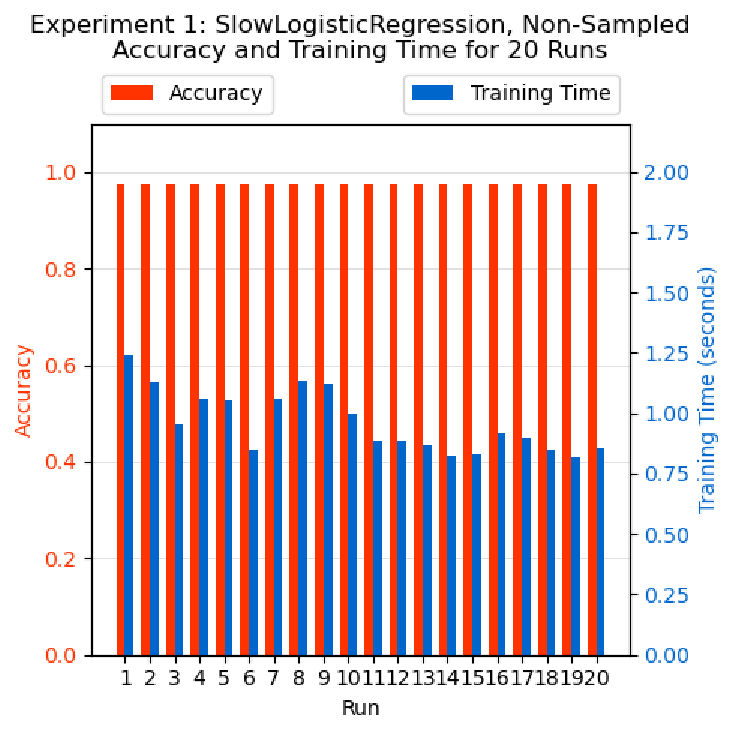
\includegraphics[width=\columnwidth]{experiment_1a}}
\caption{Measured accuracies and training times observed over 20 training cycles of \texttt{SlowLogisticRegression}, without any sampling, using the Breast Cancer Wisconsin Diagnostic Dataset \cite{breastcancer}.}
\label{experiment_1a}
\end{center}
\vskip -0.2in
\end{figure}

\begin{figure}[ht]
\vskip 0.2in
\begin{center}
\centerline{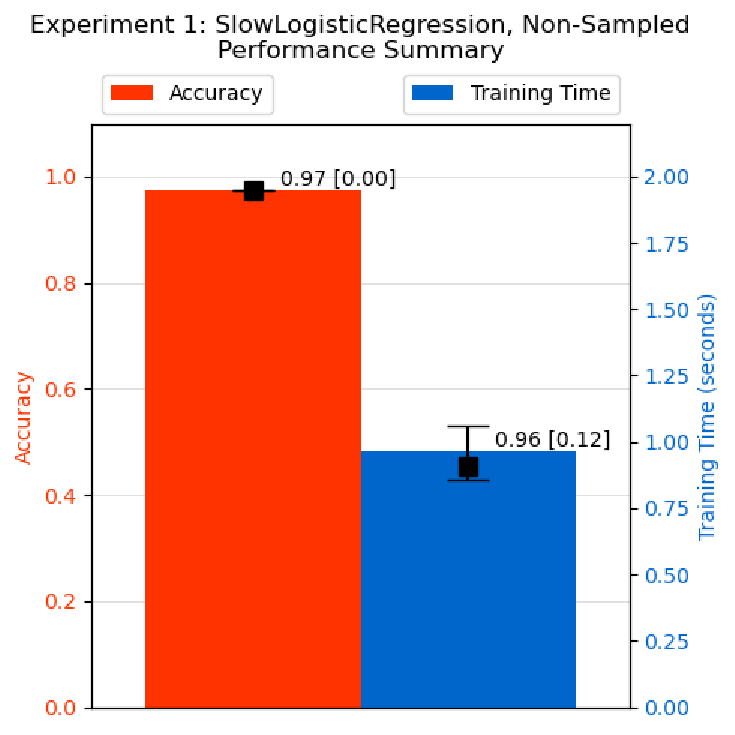
\includegraphics[width=\columnwidth]{experiment_1b}}
\caption{Mean accuracies and training times observed over 20 training cycles of \texttt{SlowLogisticRegression}, without any sampling, using the Breast Cancer Wisconsin Diagnostic Dataset \cite{breastcancer}.}
\label{experiment_1a}
\end{center}
\vskip -0.2in
\end{figure}


\begin{figure}[ht]
\vskip 0.2in
\begin{center}
\centerline{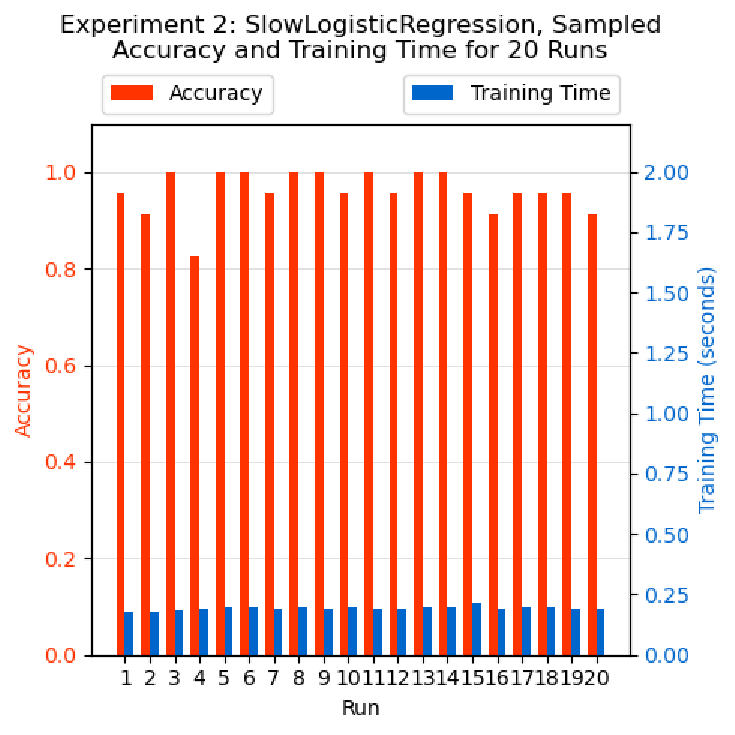
\includegraphics[width=\columnwidth]{experiment_2a}}
\caption{Measured accuracies and training times observed over 20 training cycles of \texttt{SlowLogisticRegression}, with \texttt{BasicLeverageScoresSampler} sampling, using the Breast Cancer Wisconsin Diagnostic Dataset \cite{breastcancer}.}
\label{experiment_1a}
\end{center}
\vskip -0.2in
\end{figure}


\begin{figure}[ht]
\vskip 0.2in
\begin{center}
\centerline{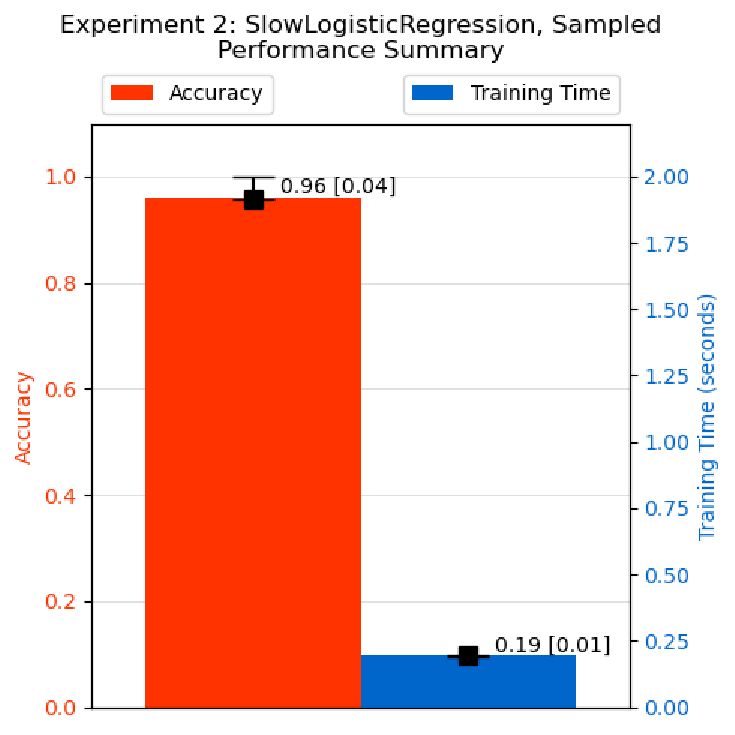
\includegraphics[width=\columnwidth]{experiment_2b}}
\caption{Measured accuracies and training times observed over 20 training cycles of \texttt{SlowLogisticRegression}, with \texttt{BasicLeverageScoresSampler} sampling, using the Breast Cancer Wisconsin Diagnostic Dataset \cite{breastcancer}.}
\label{experiment_1a}
\end{center}
\vskip -0.2in
\end{figure}


\begin{figure}[ht]
\vskip 0.2in
\begin{center}
\centerline{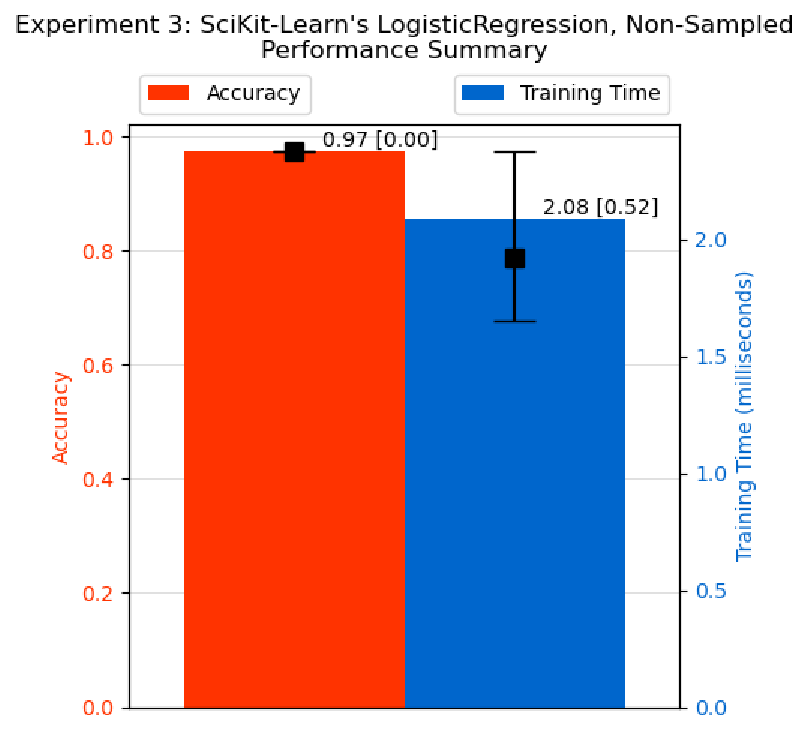
\includegraphics[width=\columnwidth]{experiment_3b}}
\caption{Mean accuracies and training times observed over 20 training cycles of SciKit-Learn's \texttt{LogisticRegression} class, without any sampling, using the Breast Cancer Wisconsin Diagnostic Dataset \cite{breastcancer}.}
\label{experiment_1a}
\end{center}
\vskip -0.2in
\end{figure}

\begin{figure}[ht]
\vskip 0.2in
\begin{center}
\centerline{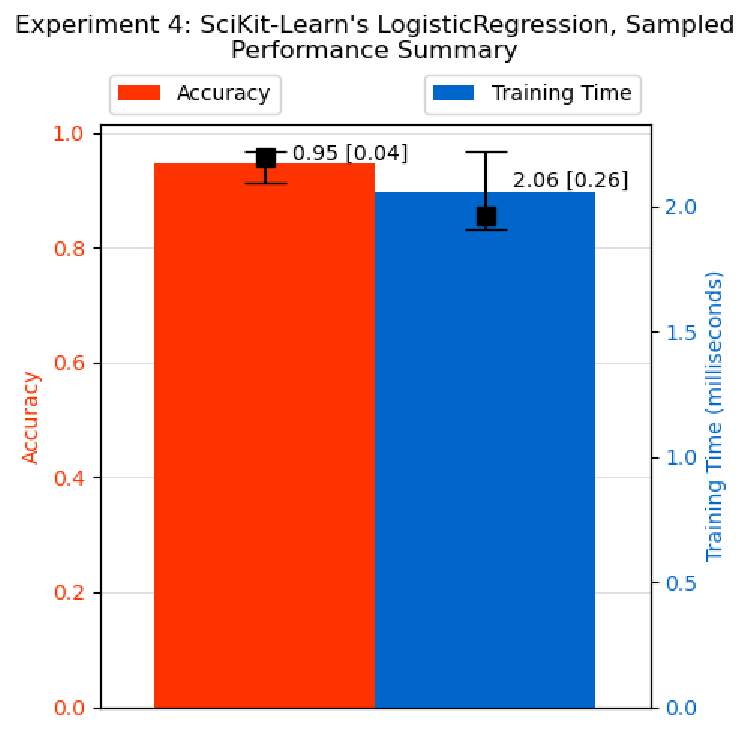
\includegraphics[width=\columnwidth]{experiment_4b}}
\caption{Mean accuracies and training times observed over 20 training cycles of SciKit-Learn's \texttt{LogisticRegression} class, with \texttt{BasicLeverageScoresSampler} sampling, using the Breast Cancer Wisconsin Diagnostic Dataset \cite{breastcancer}.}
\label{experiment_1a}
\end{center}
\vskip -0.2in
\end{figure}

\begin{figure}[ht]
\vskip 0.2in
\begin{center}
\centerline{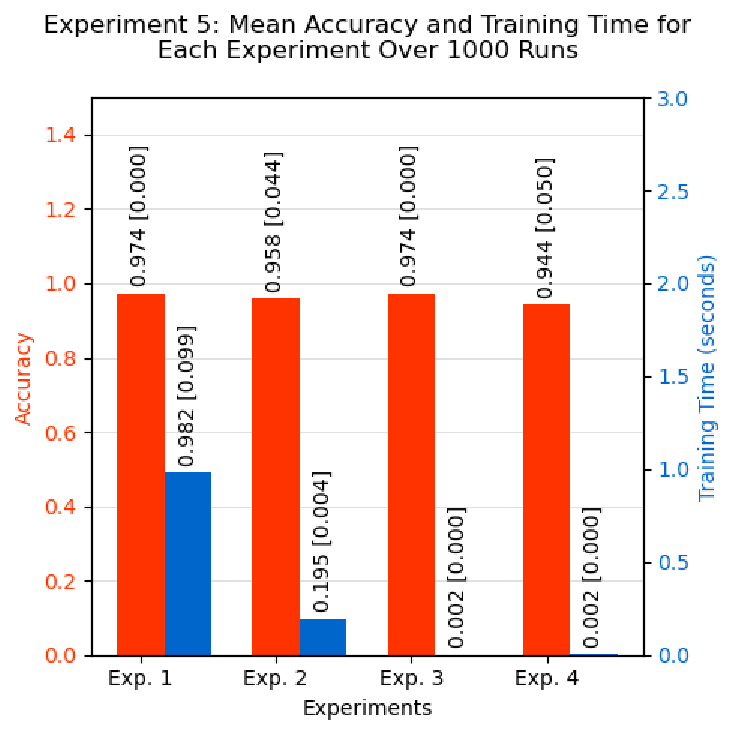
\includegraphics[width=\columnwidth]{experiment_5}}
\caption{Mean accuracies and training times observed when repeating experiments 1, 2, 3, and 3, this time with 1000 training cycles each.}
\label{experiment_1a}
\end{center}
\vskip -0.2in
\end{figure}


\subsection{Next Steps}

In light of the positive preliminary results observed in this initial exploratory phase, we propose the following next steps to give continuity to this study:
\begin{itemize}

 \item \textbf{Complete Sampling Algorithm Implementation:} As stated earlier, this preliminary exploration implemented a simplified version of the algorithm proposed by \citeauthor{chow24}. To provide more depth and substance to this study, a full implementation of the algorithm is necessary. This effort will allow for more comprehensive benchmarking and trade-off analysis, as well as a better understanding of the circumstances in which the different variations demonstrate better (or worse) employability.

\item \textbf{Use-Case Diversification:} \citeauthor{chow24} focus their work on logistic regression models. Given that dataset reduction is a topic of common interest in the Machine Learning field, an exploration of whether the sampling algorithms implemented in this project can be used to train other types of prediction models is justified. Therefore, we propose a more substantial analysis into this question as a natural next step for this study.

\end{itemize}


\subsection{Proposal for Course Project}

\subsubsection{Overview}

Our proposal for this study is multifold. Ultimately, we aim to provide (1) an implementation of the full sampling algorithm as originally proposed by \citeauthor{chow24}, (2) a simplified version that aims to strike a reasonable balance between computational performance and prediction accuracy, and (3) an empirical evaluation of the technical feasibility of employing the sampling algorithms implemented here on the training process of other types of prediction models beyond logistic regression.

\subsubsection{Methodology}

To achieve the aforementioned goals, a thorough benchmark is necessary to evaluate how the simplified algorithm performs relative to the full implementation in diverse datasets. To keep comparisons objective, we will focus on select metrics such as \textbf{accuracy} ($Acc$),  \textbf{non-sampled training time} ($t_{ns}$, the time taken to train a model on the full dataset), and \textbf{sampled training time} ($t_s$,  the time taken to train a model with sampled data, including sampling time).

Formally, we define:
$$
Acc(y, \hat{y}) = \frac{1}{n} \sum_{i=0}^{n-1} 1(\hat{y}_i = y_i)
$$

And

$$
t_s = s + t
$$

Where:

\begin{itemize}

\item[$y$] is a vector representing the true values.
\item[$\hat{y}$] is a vector representing the predictions.
\item[$n$] is the number of predictions based on which accuracy is being calculated.
\item[$s$] is the time consumed by the sampling algorithm to derive a reduced dataset.

\end{itemize}

Moreover, each algorithm-dataset combination will be run an adequate number of times for statistical relevance, and the key metrics are to be captured each time. Performance comparisons will be made with average values. This practice will allow for more consistent performance analysis across implementations. Specifically, the simplified and complete versions of the algorithms will be tested with different databases, such as those used by \citeauthor{chow24}, and also well-known open-source datasets, such as the Breast Cancer Wisconsin Diagnostic Data Set \cite{breastcancer}, among others. Further information regarding experiment design details are included in Appendix A.

Lastly, we will assess whether the sampling algorithms contribute positively or negatively when used to train different prediction models beyond binary classification. At this preliminary stage, the types of predictions scoped for further exploration are \textbf{to be defined}.


\subsubsection{Feasibility}

Given the empirical nature of this study, the project so far has demonstrated to be technically feasible, from an implementation standpoint. The paper \cite{chow24} provides a thorough review of the mathematical background, as well as detailed information behind the algorithm's rationale and theoretical foundations. Additionally, the authors provide their own implementation in Python code, which is publicly available and may be used for benchmarking as part of this study.


\subsubsection{Relevance}

Our literature review indicates numerous efforts in the machine learning community in pushing the barriers of predictive algorithms, and in seeking creative solutions to improve accuracy and optimize computational efficiency of known methods. In particular, the core contribution of this project involves addressing questions left open by \citeauthor{chow24}, such as (1) are the theoretical guarantees provided by the original implementation indispensible, or could a simplified version of the algorithm provide comparable performance? And (2) can this sample method contribute positively to the training process of different machine learning models? By addressing these questions, our work further expands the body of knowledge proposed by the authors, and provides the academic community with further insights into the use of randomized sampling algorithms in reducing large training datasets.


\section{Conclusion}

...


\section*{Software and Data}

Download links to the code that accompanies this study to be provided after the anonymous peer review.

\section*{Impact Statement}

...

Authors are \textbf{required} to include a statement of the potential 
broader impact of their work, including its ethical aspects and future 
societal consequences. This statement should be in an unnumbered 
section at the end of the paper (co-located with Acknowledgements -- 
the two may appear in either order, but both must be before References), 
and does not count toward the paper page limit. In many cases, where 
the ethical impacts and expected societal implications are those that 
are well established when advancing the field of Machine Learning, 
substantial discussion is not required, and a simple statement such 
as the following will suffice:

``This paper presents work whose goal is to advance the field of 
Machine Learning. There are many potential societal consequences 
of our work, none which we feel must be specifically highlighted here.''


\bibliography{paper_references}
\bibliographystyle{icml2025}


%%%%%%%%%%%%%%%%%%%%%%%%%%%%%%%%%%%%%%%%%%%%%%%%%%%%%%%%%%%%%%%%%%%%%%%%%%%%%%%
%%%%%%%%%%%%%%%%%%%%%%%%%%%%%%%%%%%%%%%%%%%%%%%%%%%%%%%%%%%%%%%%%%%%%%%%%%%%%%%
% APPENDIX
%%%%%%%%%%%%%%%%%%%%%%%%%%%%%%%%%%%%%%%%%%%%%%%%%%%%%%%%%%%%%%%%%%%%%%%%%%%%%%%
%%%%%%%%%%%%%%%%%%%%%%%%%%%%%%%%%%%%%%%%%%%%%%%%%%%%%%%%%%%%%%%%%%%%%%%%%%%%%%%
\newpage
\appendix
\onecolumn
\section{Experiments}

\subsubsection{Objective Metrics}

The goal of the experiment described here is to record key metrics for each model-dataset combination, namely \textbf{accuracy} ($Acc$), \textbf{non-sampled training time} ($t_{ns}$, the time taken to train a model on the full dataset), and \textbf{sampled training time} ($t_s$,  the time taken to train a model with sampled data, including sampling time).

Formally, we define:
$$
Acc(y, \hat{y}) = \frac{1}{n} \sum_{i=0}^{n-1} 1(\hat{y}_i = y_i)
$$

And

$$
t_s = s + t
$$

Where:

\begin{itemize}

\item[$y$] is a vector representing the true values.
\item[$\hat{y}$] is a vector representing the predictions.
\item[$n$] is the number of predictions based on which accuracy is being calculated.
\item[$s$] is the time consumed by the sampling algorithm to derive a reduced dataset.

\end{itemize}

Additionally, each experiment defines its own set of parameters and leverage different algorithm implementations.

\subsection{Experiment 1: \texttt{SlowLogisticRegression}'s Performance, No Sampling}


\subsubsection{Objective}

The experiment aims to assess the performance of a custom implementation of logistic regression, named \texttt{SlowLogisticRegression}, in terms of classification accuracy and training time across multiple runs on an open-source dataset \cite{breastcancer}. The experiment seeks to quantify the model's generalization ability and computational efficiency under standardized conditions.


\subsubsection{Materials and Methods}

The experiment utilizes a dataset represented by feature matrix $ X \in \mathbb{R}^{n \times m} $ and target vector $ y \in \{0, 1\}^n $, where $ n $ is the number of samples and $ m $ is the number of features. The dataset is assumed to be preprocessed and suitable for binary classification tasks.

For each experimental run, the dataset is split into training and test sets using an 80-20 partition, with 80\% of the data allocated to training ($ X_{\text{train}}, y_{\text{train}} $) and 20\% to testing ($ X_{\text{test}}, y_{\text{test}} $). The split is performed using a fixed random seed of 42 to ensure reproducibility across runs. Feature scaling is applied using Python's SciKit-Learn \texttt{MinMaxScaler}, which normalizes each feature to the range $[0, 1]$ based on the training set's minimum and maximum values. The scaling transformation is computed as:
$$
X'_{i,j} = \frac{X_{i,j} - \min(X_{:,j})}{\max(X_{:,j}) - \min(X_{:,j})}
$$

where $ X_{i,j} $ denotes the $ j $-th feature of the $ i $-th sample, and the transformation is fitted on $ X_{\text{train}} $ and applied to both $ X_{\text{train}} $ and $ X_{\text{test}} $.


\subsubsection{Model and Training}

The classification model employed is a custom logistic regression implementation (\texttt{SlowLogisticRegression}), parameterized by a learning rate of 0.1 and a fixed number of 5000 training epochs. The implementation of this model is detailed in section 2 of this paper.


\subsubsection{Experimental Procedure}

The experiment is repeated 20 times for this experiment. For each iteration:

\begin{itemize}
 \item [1.] The dataset is split into training and test sets.
 \item [2.] Features are scaled using \texttt{MinMaxScaler}.
 \item [3.] The \texttt{SlowLogisticRegression} model is initialized and trained on the scaled training data, with training time recorded.
 \item [4.] Predictions are generated on the scaled test set.
 \item [5.] Accuracy is calculated by comparing predictions to the true test labels.
 \item [6.] Accuracy and training time are tracked separately.
\end{itemize}

This procedure records the accuracy scores and training times across each cycle, which are later used to calculate the average values for each metric.


\subsubsection{Analysis}

The collected accuracies and training times enable statistical analysis of the model's performance. Key statistics, such as the mean and standard deviation of accuracy, can be computed to evaluate consistency and generalization. Similarly, training time statistics provide insight into the computational cost of the \texttt{SlowLogisticRegression} implementation without any sampling.


\subsubsection{Assumptions and Limitations}

The experiment assumes that the dataset is suitable for binary classification and that the features benefit from min-max scaling. The fixed hyperparameters (learning rate = 0.1, epochs = 5000), obtained empirically, appear to suit this experiment well and provide satisfactory results.


\subsubsection{Expected Outcomes}

The experiment is expected to yield a distribution of accuracy scores reflecting the model's predictive capability and a distribution of training times indicating its efficiency. These results can be used to benchmark \texttt{SlowLogisticRegression} against other implementations or algorithms under identical conditions.



\subsection{Experiment 2: \texttt{SlowLogisticRegression}'s Performance with Leverage Score Sampling}

\subsubsection{Objective}

The experiment aims to assess the performance of a custom implementation of logistic regression, named \texttt{SlowLogisticRegression}, in terms of classification accuracy and training time across multiple runs on an open-source dataset \cite{breastcancer}. The experiment seeks to quantify the model's generalization ability and computational efficiency under standardized conditions, incorporating a data sampling step using the randomized sampling algorithm \texttt{BasicLeverageScoresSampler}.


\subsubsection{Materials and Methods}

The experiment utilizes a dataset represented by feature matrix $ X \in \mathbb{R}^{n \times m} $ and target vector $ y \in \{0, 1\}^n $, where $ n $ is the number of samples and $ m $ is the number of features. The dataset is assumed to be preprocessed and suitable for binary classification tasks.

For each experimental run, the dataset is first sampled to 20\% of its original size using the \texttt{BasicLeverageScoresSampler}, resulting in a reduced dataset ($ X_{\text{sampled}}, y_{\text{sampled}} $). This sampled dataset is then split into training and test sets using an 80-20 partition, with 80\% of the sampled data allocated to training ($ X_{\text{train}}, y_{\text{train}} $) and 20\% to testing ($ X_{\text{test}}, y_{\text{test}} $). The split is performed using a fixed random seed of 42 to ensure reproducibility across runs. Feature scaling is applied using Python's SciKit-Learn \texttt{MinMaxScaler}, which normalizes each feature to the range $[0, 1]$ based on the training set's minimum and maximum values. The scaling transformation is computed as:
\[
X'_{i,j} = \frac{X_{i,j} - \min(X_{:,j})}{\max(X_{:,j}) - \min(X_{:,j})}
\]
where $ X_{i,j} $ denotes the $ j $-th feature of the $ i $-th sample, and the transformation is fitted on $ X_{\text{train}} $ and applied to both $ X_{\text{train}} $ and $ X_{\text{test}} $.

\subsubsection{Model and Training}

The classification model employed is a custom logistic regression implementation (\texttt{SlowLogisticRegression}), parameterized by a learning rate of 0.1 and a fixed number of 5000 training epochs. The implementation of this model is detailed in section 2 of this paper.

\subsubsection{Experimental Procedure}

The experiment is repeated 20 times for this experiment. For each iteration:

\begin{itemize}
 \item [1.] The dataset is sampled to 20\% of its original size using \texttt{BasicLeverageScoresSampler}.
 \item [2.] The sampled dataset is split into training and test sets.
 \item [3.] Features are scaled using \texttt{MinMaxScaler}.
 \item [4.] The \texttt{SlowLogisticRegression} model is initialized and trained on the scaled training data, with training time recorded.
 \item [5.] Predictions are generated on the scaled test set.
 \item [6.] Accuracy is calculated by comparing predictions to the true test labels.
 \item [7.] Accuracy and training time are tracked separately.
\end{itemize}

This procedure records the accuracy scores and training times across each cycle, which are later used to calculate the average values for each metric.

\subsubsection{Analysis}

The collected accuracies and training times enable statistical analysis of the model's performance. Key statistics, such as the mean and standard deviation of accuracy, can be computed to evaluate consistency and generalization. Similarly, training time statistics provide insight into the computational cost of the \texttt{SlowLogisticRegression} implementation with leverage score sampling.

\subsubsection{Assumptions and Limitations}

The experiment assumes that the dataset is suitable for binary classification and that the features benefit from min-max scaling. The fixed hyperparameters (learning rate = 0.1, epochs = 5000), obtained empirically, appear to suit this experiment well and provide satisfactory results. Additionally, the use of leverage score sampling assumes that the selected 20\% subset adequately represents the original dataset's structure.

\subsubsection{Expected Outcomes}

The experiment is expected to yield a distribution of accuracy scores reflecting the model's predictive capability and a distribution of training times indicating its efficiency. These results can be used to benchmark \texttt{SlowLogisticRegression} against other implementations or algorithms under identical conditions, and particularly to evaluate the impact of leverage score sampling algorithm \texttt{BasicLeverageScoresSampler} impacts on prediction accuracy and model training time.


\subsection{Experiments 3 and 4: Repeating Experiments 1 and 2 using SciKit-Learn's \texttt{LogisticRegression} Model}

\subsubsection{Objective}

Experiments 3 and 4 replicate Experiments 1 and 2, respectively, replacing \texttt{SlowLogisticRegression} with SciKit-Learn's optimized \texttt{LogisticRegression} class. Experiment 3 uses the full dataset, while Experiment 4 applies 20\% leverage score sampling via \texttt{BasicLeverageScoresSampler}. The goal is to assess whether sampling impacts the performance of an optimized model, comparing accuracy and training efficiency against Experiments 1 and 2 to evaluate sampling effects across custom and optimized implementations.

\subsubsection{Materials and Methods}

The dataset, sampling (for Experiment 4), and scaling follow the procedures in Experiments 1 and 2, using $ X \in \mathbb{R}^{n \times m} $, $ y \in \{0, 1\}^n $, an 80-20 train-test split (random seed 42), and \texttt{MinMaxScaler} normalization.

\subsubsection{Model and Training}

The model is SciKit-Learn's \texttt{LogisticRegression} with default parameters, replacing the custom \texttt{SlowLogisticRegression} (learning rate 0.1, 5000 epochs) used previously.

\subsubsection{Experimental Procedure}

The experiment is repeated 20 times per condition. The same procedure detailed for previous experiments are employed here for Experiment 3 and 4.

\subsubsection{Analysis}

Mean and standard deviation of accuracy and training times assess consistency, generalization, and computational cost, comparing optimized \texttt{LogisticRegression} performance with and without sampling.

\subsubsection{Assumptions and Limitations}

The experiment assumes binary classification suitability and effective min-max scaling. Default \texttt{LogisticRegression} parameters are presumed optimal, and sampling assumes the 20\% subset retains dataset structure.

\subsubsection{Expected Outcomes}

Accuracy and training time distributions will reveal \texttt{LogisticRegression}'s performance, highlighting sampling impacts versus Experiments 1 and 2, and benchmarking optimized versus custom models.


\subsection{Experiment 5: Statistical Validation of Experiments 1–4 with Increased Runs}

\subsubsection{Objective}

Experiment 5 re-executes Experiments 1, 2, 3, and 4, increasing the number of cycles from 20 to 1000 per condition, to enhance the statistical relevance of prior observations. It assesses \texttt{SlowLogisticRegression} and \texttt{LogisticRegression} performance under full and 20\% sampled dataset scenarios, aiming to confirm the consistency and reliability of accuracy and training time findings from earlier experiments.

\subsubsection{Materials and Methods}

The dataset, sampling (for Experiments 2 and 4), and scaling remain as in Experiments 1–4, using $ X \in \mathbb{R}^{n \times m} $, $ y \in \{0, 1\}^n $, an 80-20 train-test split (random seed 42), and \texttt{MinMaxScaler} normalization.

\subsubsection{Model and Training}

Models are \texttt{SlowLogisticRegression} (learning rate 0.1, 5000 epochs) for Experiments 1 and 2, and SciKit-Learn's \texttt{LogisticRegression} (default parameters) for Experiments 3 and 4, as previously defined.

\subsubsection{Experimental Procedure}

The experiment is repeated 1000 times per condition (Experiments 1–4). The same procedures described earlier for each experiment still apply here.

\subsubsection{Analysis}

Mean and standard deviation of accuracy and training times, based on 1000 runs, provide robust statistical validation of consistency, generalization, and computational cost across all conditions.

\subsubsection{Assumptions and Limitations}

Assumptions align with Experiments 1–4: binary classification suitability, effective scaling, and representative sampling. Fixed parameters for \texttt{SlowLogisticRegression} and defaults for \texttt{LogisticRegression} are presumed suitable.

\subsubsection{Expected Outcomes}

Distributions of accuracy and training times across 1000 runs will confirm the statistical relevance of Experiments 1–4, reinforcing comparisons between models and sampling effects with greater confidence.


%%%%%%%%%%%%%%%%%%%%%%%%%%%%%%%%%%%%%%%%%%%%%%%%%%%%%%%%%%%%%%%%%%%%%%%%%%%%%%%
%%%%%%%%%%%%%%%%%%%%%%%%%%%%%%%%%%%%%%%%%%%%%%%%%%%%%%%%%%%%%%%%%%%%%%%%%%%%%%%


\end{document}
